\section{Segmentation}

Segmentation is the challenge of taking a given image or scene and extracting individual objects or `components'.

Typically this can be a complex problem to tackle as stafflines connect almost all components together and must therefore first be removed. Also some musical entities are themselves comprised of multiple other entities. Good examples are the bass clef which is comprised of two dots placed above each other to the right of the curve (\cref{sec:music-theory-clefs}) and dotted notes (\cref{table:note-lengths}).

Particularly in this project, we also need to be able to break down the musical entities further into stems and note heads and so separating these from each other present another problem which we must take into account.

\subsection{Connected Component Analysis}

Connected component analysis is a technique used to establish distinct regions within an image. An individual pixel in a binary image can possess two forms of connectedness, \emph{4-neighbour} or \emph{8-neighbour}. It should be noted that this evaluation only takes place for pixels with a value of 1 or ``filled pixels''.

More formally, ``A connected component labelling of a binary image B is a labeled image LB in which the value of each pixel is the label of it's connected component'' \parencite[pg 69]{shapiro2001computer}

To be \textbf{4-neighbour}, at least one of the pixels above, below or to the left or right (which we can refer to as the vertical and horizontal neighbours) of the pixel under investigation must have a value of 1.

In a similar fashion, an \textbf{8-neighbour} pixel is one where any of the surrounding 8 pixels (vertical, horizontal or diagonal neighbours) has a value of 1.

Regions for 4-neighbour and 8-neighbour connected pixels are outlined in \cref{fig:pixel-neighbours}

\begin{figure}[h!]
    \centering
    \begin{subfigure}[b]{.6\linewidth}
        \centering
        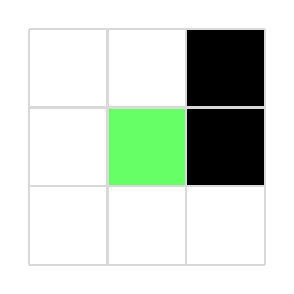
\begin{tikzpicture}
  \fill[green!60] (1,1) rectangle (2,2);
  \fill[black] (2,1) rectangle (3,2);
  \fill[black] (2,2) rectangle (3,3);
  \draw[thick,step=1cm,color=gray!30] (0, 0) grid (3,3);
\end{tikzpicture}

        \caption{Image (The pixel being examined is higlighted)}
    \end{subfigure}

    \vspace*{0.5in}

    \begin{subfigure}[b]{.4\linewidth}
        \centering
        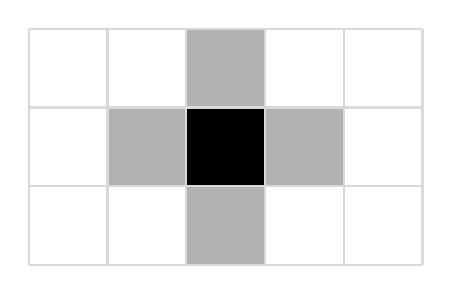
\begin{tikzpicture}
  \fill[black] (1,1) rectangle (2,2);
  \fill[gray!60]  (1,0) rectangle (2,1);
  \fill[gray!60]  (0,1) rectangle (1,2);
  \fill[gray!60]  (2,1) rectangle (3,2);
  \fill[gray!60]  (1,2) rectangle (2,3);
  \draw[thick,step=1cm,color=gray!30] (-1, 0) grid (4,3);
\end{tikzpicture}

        \caption{4 Neighbour Regions}
        \label{fig:4-neighbour-regions}
    \end{subfigure}
    \begin{subfigure}[b]{.4\linewidth}
        \centering
        \input{gfx/background-omr/connected-component/neighbour-4-connected.tikz}
        \caption{4N - 2 Regions Identified}
        \label{fig:4-neighbour-regions}
    \end{subfigure}

    \vspace*{0.5in}

    \begin{subfigure}[b]{.4\linewidth}
        \centering
        \input{gfx/background-omr/connected-component/neighbour-8.tikz}
        \label{fig:8-neighbour-regions}
        \caption{8 Neighbour Regions}
    \end{subfigure}
    \begin{subfigure}[b]{.4\linewidth}
        \centering
        \input{gfx/background-omr/connected-component/neighbour-8-connected.tikz}
        \label{fig:8-neighbour-connected}
        \caption{8N - 1 Region Identified}
    \end{subfigure}

    \caption{4 and 8 Neighbour Regions and examples of connected pixels}
    \label{fig:pixel-neighbours}
\end{figure}

There are two primary algorithms for establishing connected regions, the first is recursive and the second requires two scans.

\subsubsection{Recursive Labelling}

If we assume that the size of the image to be evaluated is small and we can fit it in memory (a reasonable assumption give the scope of the project and the hardware available) we can employ a recursive algorithm which can grow regions by visiting any pixel in the image using depth first of breadth first searching. An outline for a depth first algorithm is given in algorithm \cref{alg:ccl-recursive}

\begin{lstlisting}[caption=Recursive Connected Component Labelling (DFS), label=alg:ccl-recursive]
let img be the binary image
let lblimg be the labelled image

lblimg = negate(image)
lbl = 0

label_components():
  for i = 0 to height:
    for j = 0 to width:
      if lblimg[i, j] == -1:
        lbl += 1
        label\_region(i, j)

label_region(i, j):
  lblimg[i, j] = lbl
  for (i', j') in neighbours(i, j):
    if lblimg[i, j] == -1:
      label_region(i', j')
\end{lstlisting}

\subsubsection{Two Pass Labelling}

An alternate algorithm involves performing the labelling in two passes. Assuming 8-neighbour connectedness and that we will most likely be scanning left to right we inspect the 3 pixels above and the pixel to the left of the current pixel as seen in \cref{fig:scan-neighbours}.

\begin{figure}[h!]
  \centering
  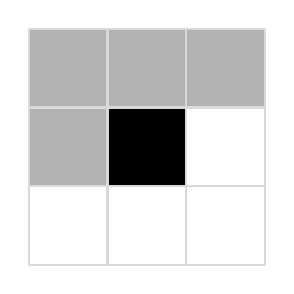
\begin{tikzpicture}

  \fill[white] (0,0) rectangle (1,1);
  \fill[white] (1,0) rectangle (2,1);
  \fill[white] (2,0) rectangle (3,1);

  \fill[gray!60] (0,1) rectangle (1,2);
  \fill[black] (1,1) rectangle (2,2);
  \fill[white] (2,1) rectangle (3,2);

  \fill[gray!60] (0,2) rectangle (1,3);
  \fill[gray!60] (1,2) rectangle (2,3);
  \fill[gray!60] (2,2) rectangle (3,3);
  \draw[thick,step=1cm,color=gray!30] (0, 0) grid (3,3);
\end{tikzpicture}

  \caption{Pixels which are inspected during each row scan}
  \label{fig:scan-neighbours}
\end{figure}

We label each pixel according to these neighbours (if neighbours have multiple labels we just pick any of them and record that they were adjacent) and then finally reduce the number of labels by merging adjacent labels. An visual example of the process can be seen in \cref{fig:ccl-two-pass}

\begin{lstlisting}[caption=Iterative Two-Pass Connected Component Labelling, label=alg:ccl-iterative]
let img be the binary image
let lblimg be the labelled image

lblimg = negate(image)
lbl = 1
equivalent_labels = []

first_pass():
  for i = 0 to height:
    for j = 0 to width:
      if lblimg[i, j] == 1:
        labels = neighbour_labels(i, j)
        if size(labels) == 0:
          lbl += 1
          lblimg[i, j] = lbl
        else:
          lblimg[i, j] = labels[0]
          if size(labels) > 1:
            equivalent_labels << labels

second_pass():
    for labelgroup in equivalent_labels:
      firstlabel  = labelgroup[0]
      otherlabels = labelgroup[1..]

      for label in otherlabels:
        relabelpixels(label, firstlabel)
\end{lstlisting}

\begin{figure}[h!]
    \centering
    \begin{subfigure}[b]{\linewidth}
        \centering
        \input{gfx/background-omr/connected-component/iterative-pass-0.tikz}
        \caption{Initial Image}
    \end{subfigure}

    \vspace*{0.5in}

    \begin{subfigure}[b]{.3\linewidth}
        \centering
        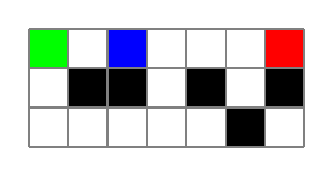
\begin{tikzpicture}

  \fill[green] (0.0,0.5) rectangle (0.5,1.5);
  \fill[white] (0.5,0.5) rectangle (1.0,1.5);
  \fill[blue] (1.0,0.5) rectangle (1.5,1.5);
  \fill[white] (1.5,0.5) rectangle (2.0,1.5);
  \fill[white] (2.0,0.5) rectangle (2.5,1.5);
  \fill[white] (2.5,0.5) rectangle (3.0,1.5);
  \fill[red] (3.0,0.5) rectangle (3.5,1.5);

  \fill[white] (0.0,0.5) rectangle (0.5,1.0);
  \fill[black] (0.5,0.5) rectangle (1.0,1.0);
  \fill[black] (1.0,0.5) rectangle (1.5,1.0);
  \fill[white] (1.5,0.5) rectangle (2.0,1.0);
  \fill[black] (2.0,0.5) rectangle (2.5,1.0);
  \fill[white] (2.5,0.5) rectangle (3.0,1.0);
  \fill[black] (3.0,0.5) rectangle (3.5,1.0);

  \fill[white] (0.0,0.0) rectangle (0.5,0.5);
  \fill[white] (0.5,0.0) rectangle (1.0,0.5);
  \fill[white] (1.0,0.0) rectangle (1.5,0.5);
  \fill[white] (1.5,0.0) rectangle (2.0,0.5);
  \fill[white] (2.0,0.0) rectangle (2.5,0.5);
  \fill[black] (2.5,0.0) rectangle (3.0,0.5);
  \fill[white] (3.0,0.0) rectangle (3.5,0.5);

  \draw[thick,step=0.5cm,color=gray] (0,0) grid (3.5,1.5);
\end{tikzpicture}

        \caption{1\textsuperscript{st} pass (Row 1)}
    \end{subfigure}
    \begin{subfigure}[b]{.3\linewidth}
        \centering
        \input{gfx/background-omr/connected-component/iterative-pass-2.tikz}
        \caption{1\textsuperscript{st} pass (Row 2)}
    \end{subfigure}
    \begin{subfigure}[b]{.3\linewidth}
        \centering
        \input{gfx/background-omr/connected-component/iterative-pass-3.tikz}
        \caption{1\textsuperscript{st} pass (Row 3)}
    \end{subfigure}

    \vspace*{0.5in}

    \begin{subfigure}[b]{.6\linewidth}
        \centering
        \input{gfx/background-omr/connected-component/iterative-pass-4.tikz}
        \caption{2\textsuperscript{nd} Pass}
    \end{subfigure}

  \caption{Step by step two pass connected component labelling}
  \label{fig:ccl-two-pass}
\end{figure}


\subsection{Projections}
\label{sec:projections}

Projections are regularly used in OMR during the preprocessing stage to detect and remove staff lines \parencite{rossant2002global}, but can also be used during the segmentation stage. An example section of score is shown in \cref{fig:stave-projection} along with it's horizontal and vertical projections.

The technique essentially involves projecting the manuscript in the x and y axes, collecting the pixels in either individual pixel lines or buckets in order to help establish information about the image.

Mathematically, if the image is represented as a 1 bit (2 colour) image $I(x_{\text{max}}, y_{\text{max}})$ of width $x_{\text{max}}$ and height $y_{\text{max}}$, let $p_{xy} \in 0, 1$ denotes the value for a specific pixel at row $y$ column $x$.

The horizontal and vertical projections can then be defined as:


\begin{lequation} \label{eq:hproj}
  P_{\text{horizontal}}(y) = \sum_{j = 0}^{x_\text{max}} p_{jy}
\end{lequation}

\begin{lequation} \label{eq:vproj}
  P_{\text{vertical}}(x) = \sum_{j = 0}^{y_\text{max}} p_{xj}
\end{lequation}

\begin{figure}[H]
  \centering
  \includegraphics[width=\linewidth]{gfx/background-omr/projection.png}
  \caption{Horizontal and Vertical Projections of handwritten music excerpt}
  \label{fig:stave-projection}
\end{figure}


\subsection{Template Matching}
\label{sec:template-matching}
Image segmentation using template matching is uncommon but not unheard of, it receives particular attention in the segmentation phase in \cite{rossant2002global}. Different templates of reference components can be matched to the score, where a high correlation score in a certain position acts as both segmentation and classification.

In testing, I was able to reproduce this effect by extracting components like the note head from the whole note as seen in Figure \cref{fig:templatematch}. However, as noted by \citeauthor{rossant2002global} this method is highly dependent on the font used in a printed score so for the purposes of handling handwritten notation it's unlikely to yield great results. Indeed, in preliminary testing, getting regular correct matches in a handwritten score proved troublesome.

\begin{figure}[h!]
  \includegraphics[width=0.6\linewidth]{gfx/template.png}
  \centering
  \caption{Example of extracting note heads using template matching utilising OpenCV and the sum of square differences scoring measure}
  \label{fig:templatematch}
\end{figure}

More formally, for the example in \cref{fig:templatematch}, template matching involves analysing each pixel in an image (or a region of an image) and comparing it to a reference pixel in a template image. The score for two $n \times m$ images $x$ and $y$ can be generated using \cref{eqn:ssd}.

\begin{lequation}\label{eqn:ssd}
  SSD_{xy} = \sum_{i = 0}^m \sum_{j = 0}^n (x(i, j) - y(i, j))^2
\end{lequation}


In the example given above, we're only looking for a subsection or a partial template so if image $x$ is $m \times n$ and image $y$ is $a \times b$ in size where $m \le a \land n \le b$, we can search each possible position $(k, l)$ for $y$ in $x$ with \cref{eqn:ssd-template}.

\begin{lequation}\label{eqn:ssd-template}
SSD_{xy}(k, l) = \sum_{i = k}^{m + k} \sum_{j = l}^{n + l} (x(i, j + l) - y(i, j))^2
\end{lequation}

and whichever positioning gives us the highest score is likely to be the best match.

\subsection{Defects and Difficulties}

There are two regular types of error that can cause issues during segmentation, \textbf{touching objects} and \textbf{broken objects}. Since these are likely to occur a lot more regularly given the freedom allowed by handwritten music and the a beginner's learning curve, it is important that the application is able to spot (and subsequently feed back on) these errors.

\subsubsection{Touching Objects}

Touching objects are where what were intended to be two separate objects actually touch and this can cause issues when segmenting components using connected component analysis \cref{sec:connected-component-analysis}. 

In a printed score, you can use \cref{sec:template-matching} template matching in order to separate the components but when they are handwritten, it's more likely we will have to rely on using vertical and horizontal projections to find the point of minimal intersection as in \cite{fujinaga1996adaptive}.
